\alt<article>{\chapter{Semantic 3DGS}}{\section{Semantic 3DGS}}
\alt<article>{\section{Overview}}{\subsection{Overview}}

\begin{frame}
	\Frametitle{Research Background}
	\colorlet{accepted}{ForestGreen}
	\alt<presentation>{
		\blfootnote{\textcolor{accepted}{Accepted by top conferences.}}
	}{
		\par Figure~\ref{fig:semantic-3dgs-timeline} shows the status of research on ``semantic 3DGS''.
	}
	\begin{figure}[htbp]
		\centering
		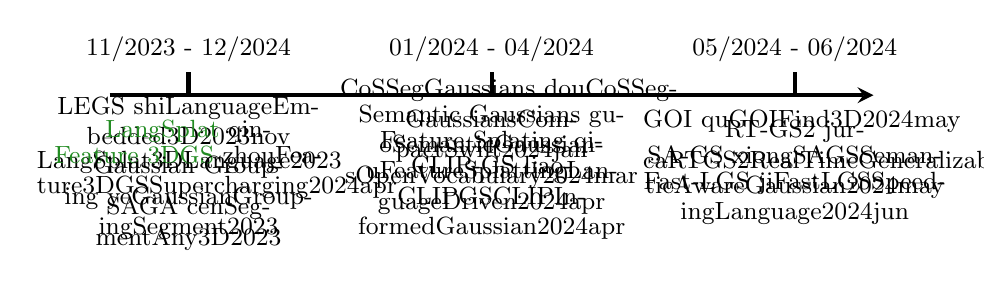
\begin{tikzpicture}
			\usetikzlibrary{calc}
			\usetikzlibrary{positioning}

			\pgfmathsetmacro{\dy}{0.3cm/1pt};
			\pgfmathsetmacro{\nodeNum}{3};
			\pgfmathsetmacro{\sepNum}{\nodeNum-1};
			\pgfmathsetmacro{\length}{0.8*\linewidth};
			\pgfmathsetmacro{\edgeLength}{1cm/1pt};
			\pgfmathsetmacro{\dx}{(\length-\edgeLength-\edgeLength)/\sepNum};
			\pgfmathsetmacro{\xShift}{0};

			\mode<presentation>{\tikzset{
					node distance=1.5ex,
					note/.style={ anchor=north, align=center, text width=\dx, yshift=-\dy/3, font={\scriptsize} },
					time/.style={ anchor=south, font={\scriptsize} }
				}}
			\mode<article>{\tikzset{
					node distance=1.5ex,
					note/.style={ anchor=north, align=center, text width=\dx, yshift=-\dy/3, font={\small} },
					time/.style={ anchor=south, font={\small} }
				}}

			\coordinate (start) at (0 pt,0 pt);
			\coordinate (end) at (\length pt,0 pt);
			\draw [line width=1.5pt,-stealth] (start) -- (end);

			\foreach \counter in {0,...,\sepNum} {
					\coordinate (s\counter) at (\edgeLength+\counter*\dx pt,0);
					\coordinate (t\counter) at ($(s\counter)+(0,\dy pt)$);
					\draw [line width=1.5pt] (s\counter) -- (t\counter);
				}
			\node [time] at (t0.north) { 11/2023 - 12/2024 };
			\node [note, below of= s0]   (s0_1) {LEGS~\autocite{shiLanguageEmbedded3D2023nov}};
			\node [note, below of= s0_1] (s0_2) {\textcolor{accepted}{LangSplat}~\autocite{qinLangSplat3DLanguage2023}};
			\node [note, below of= s0_2] (s0_3) {\textcolor{accepted}{Feature 3DGS}~\autocite{zhouFeature3DGSSupercharging2024apr}};
			\node [note, below of= s0_3] (s0_4) {Gaussian Grouping~\autocite{yeGaussianGroupingSegment2023}};
			\node [note, below of= s0_4] (s0_5) {SAGA~\autocite{cenSegmentAny3D2023}};
			\node [time] at (t1.north) { 01/2024 - 04/2024 };
			\node [note, below of= s1]   (s1_1) {CoSSegGaussians~\autocite{douCoSSegGaussiansCompactSwift2024jan}};
			\node [note, below of= s1_1] (s1_2) {Semantic Gaussians~\autocite{guoSemanticGaussiansOpenVocabulary2024mar}};
			\node [note, below of= s1_2] (s1_3) {Feature Splating~\autocite{qiuFeatureSplattingLanguageDriven2024apr}};
			\node [note, below of= s1_3] (s1_4) {CLIP-GS~\autocite{liaoCLIPGSCLIPInformedGaussian2024apr}};
			\node [time] at (t2.north) { 05/2024 - 06/2024 };
			\node [note, below of= s2]   (s2_1) {GOI~\autocite{quGOIFind3D2024may}};
			\node [note, below of= s2_1] (s2_2) {RT-GS2~\autocite{jurcaRTGS2RealTimeGeneralizable2024may}};
			\node [note, below of= s2_2] (s2_3) {SA-GS~\autocite{xiongSAGSSemanticAwareGaussian2024may}};
			\node [note, below of= s2_3] (s2_4) {Fast-LGS~\autocite{jiFastLGSSpeedingLanguage2024jun}};
		\end{tikzpicture}
		\smallskip
		\caption[Timeline of Semantic 3DGS research]{Timeline of Semantic 3DGS research (\textcolor{accepted}{accepted})}\label{fig:semantic-3dgs-timeline}
	\end{figure}
	\mode<presentation>{\vspace*{\fill}}
	\begin{block}{Consensus}
		\begin{itemize}[<+(1)->]
			\mode<presentation>{\setlength{\itemsep}{1.5ex}}
			\item \alert<.(1)|handout:0>{What} do we care about?
			      \mode<presentation>{\vspace*{1.5ex}}
			      \begin{itemize}
				      \mode<presentation>{\setlength{\itemsep}{1.5ex}}
				      \item Accuracy; Consistency\footnote{to be 3D globally coherent}; Efficiency; Interactivity\footnote{manipulation, edit, localization, query, simulation, etc.}.
			      \end{itemize}
			\item \alert<.(1)|handout:0>{How} can we achieve it?
			      \mode<presentation>{\vspace*{1.5ex}}
			      \begin{itemize}
				      \mode<presentation>{\setlength{\itemsep}{1.5ex}}
				      \item Lift 2D foundation models\footnote{
					            CLIP, SAM, DINO, etc.
				            }
				            to scene-specific 3D Gaussians under 2D supervision.
			      \end{itemize}
		\end{itemize}
	\end{block}
	\mode<presentation>{
		\blfootnote{2D foundation models: CLIP, SAM, DINO, etc. }
		\blfootnote{Interactivity: manipulation, edit, localization, query, simulation, etc.}
	}
\end{frame}

\begin{frame}
	\Frametitle{Taxonomy}
	\colorlet{easy}{ForestGreen}
	\colorlet{challenging}{Cerulean}
	\colorlet{hard}{OrangeRed}
	\mode<article>{
		\par Figure~\ref{fig:semantic-3dgs-taxonomy-of-methodology-for-slam} is a taxonomy of methodologies in current semantic 3DGS research. However, the online and exploratory setting of SLAM is quite different from offline learning. The methods are tagged \textcolor{easy}{easy}, \textcolor{challenging}{challenging} and \textcolor{hard}{hard} for the setting of SLAM.
	}
	\tikzset{
		easy/.style={
				draw=easy,
			},
		challenging/.style={
				draw=challenging,
			},
		hard/.style={
				draw=hard,
			},
	}
	\begin{figure}[htbp]
		\centering
		\resizebox{0.8\textwidth}{!}{
			\begin{forest}
				for tree={
				my tree
				},
				[
				\textbf{Semantic 3DGS} [
				\textbf{Accuracy} [
				DINO\,\textcolor{blue!70}{\SnowflakeChevron},challenging [\normalfont\autocite{shiLanguageEmbedded3D2023nov,qiuFeatureSplattingLanguageDriven2024apr,douCoSSegGaussiansCompactSwift2024jan}]
				][
				SAM Feature-based Distillation\,\textcolor{blue!70}{\SnowflakeChevron},challenging [\normalfont\autocite{zhouFeature3DGSSupercharging2024apr,cenSegmentAny3D2023,qiuFeatureSplattingLanguageDriven2024apr}]
				][
				SAM Response-based Distillation\,\textcolor{blue!70}{\SnowflakeChevron},easy [\normalfont\autocite{qinLangSplat3DLanguage2023,yeGaussianGroupingSegment2023,liaoCLIPGSCLIPInformedGaussian2024apr}]
				][
				3D Prior Regularization, easy[\normalfont\autocite{yeGaussianGroupingSegment2023,cenSegmentAny3D2023}]
				][
				Spatial Feature Fusion, challenging[\normalfont\autocite{jurcaRTGS2RealTimeGeneralizable2024may,douCoSSegGaussiansCompactSwift2024jan}]
				][
				3D Segmentation, challenging[\normalfont\autocite{guoSemanticGaussiansOpenVocabulary2024mar}]
				]
				][
				\textbf{Efficiency} [
					Dimensionality Alignment, easy[\normalfont\autocite{zhouFeature3DGSSupercharging2024apr,yeGaussianGroupingSegment2023,qiuFeatureSplattingLanguageDriven2024apr}]
				][
					Index/Grid Map, easy[\normalfont\autocite{liaoCLIPGSCLIPInformedGaussian2024apr,jiFastLGSSpeedingLanguage2024jun}]
				][
					Self-supervised Embedding Compression, hard[\normalfont\autocite{liaoCLIPGSCLIPInformedGaussian2024apr,qinLangSplat3DLanguage2023,jurcaRTGS2RealTimeGeneralizable2024may}]
				]
				][
				\textbf{Consistency} [
					Zero-shot Video Tracker\,\textcolor{blue!70}{\SnowflakeChevron}, easy[\normalfont\autocite{yeGaussianGroupingSegment2023,liaoCLIPGSCLIPInformedGaussian2024apr,douCoSSegGaussiansCompactSwift2024jan}]
				][
					Multi-View Association, easy[\normalfont\autocite{jiFastLGSSpeedingLanguage2024jun}]
				][
					Multi-View Contrastive Learning, hard[\normalfont\autocite{jurcaRTGS2RealTimeGeneralizable2024may}]
				]
				]
				]
			\end{forest}
		}
		\mode<presentation>{
			\resizebox{0.1\textwidth}{!}{
				\begin{tikzpicture}
					\node [font=\bfseries] (caption node) {For SLAM};
					\node [my node for tree, draw=easy, below of = caption node] (easy node) {easy};
					\node [my node for tree, draw=challenging, below of = easy node] (challenging node) {challenging};
					\node [my node for tree, draw=hard, below of = challenging node] (hard node) {hard/unattainable};
				\end{tikzpicture}
			}
		}
        \smallskip
		\caption{Taxonomy of Semantic 3DGS}
		\label{fig:semantic-3dgs-taxonomy-of-methodology-for-slam}
	\end{figure}
\end{frame}
